\documentclass[11pt]{article}
\usepackage[margin=1in]{geometry}
\usepackage[T1]{fontenc}
\usepackage{lmodern}
\usepackage{microtype}
\usepackage{amsmath}
\usepackage{graphicx}
\usepackage{booktabs}
\usepackage[numbers,sort&compress]{natbib}
\usepackage[hidelinks]{hyperref}
\usepackage{caption}
\usepackage{placeins}
\captionsetup{font=small,labelfont=bf}

% Auto-generated by src/make_numbers.py -- do not edit by hand.
\newcommand{\nLabSpectra}{7,271}
\newcommand{\nSpecies}{2,281}
\newcommand{\nSamples}{3,760}
\newcommand{\nLabTrain}{5,691}
\newcommand{\nLabTest}{1,580}
\newcommand{\nLabTestSpecies}{790}
\newcommand{\nMarsRows}{343}
\newcommand{\nMarsMatched}{342}
\newcommand{\nMarsEval}{255}
\newcommand{\nMarsTargets}{48}
\newcommand{\pctOlivine}{47\%}
\newcommand{\majAcc}{50\%}
\newcommand{\majBal}{18\%}
\newcommand{\balCosineOpen}{19\%}
\newcommand{\balCICosineOpen}{2\%--24\%}
\newcommand{\accCosineOpen}{5\%}
\newcommand{\recCarbonateCosineOpen}{0\%}
\newcommand{\recFeldsparCosineOpen}{10\%}
\newcommand{\recOlivineCosineOpen}{0\%}
\newcommand{\recPyroxeneCosineOpen}{0\%}
\newcommand{\recSilicaCosineOpen}{88\%}
\newcommand{\recSulfateCosineOpen}{17\%}
\newcommand{\balCosineMars}{60\%}
\newcommand{\balCICosineMars}{33\%--66\%}
\newcommand{\accCosineMars}{45\%}
\newcommand{\recCarbonateCosineMars}{38\%}
\newcommand{\recFeldsparCosineMars}{80\%}
\newcommand{\recOlivineCosineMars}{36\%}
\newcommand{\recPyroxeneCosineMars}{25\%}
\newcommand{\recSilicaCosineMars}{100\%}
\newcommand{\recSulfateCosineMars}{79\%}
\newcommand{\balCosineWindowOpen}{17\%}
\newcommand{\balCICosineWindowOpen}{1\%--21\%}
\newcommand{\accCosineWindowOpen}{6\%}
\newcommand{\recCarbonateCosineWindowOpen}{9\%}
\newcommand{\recFeldsparCosineWindowOpen}{0\%}
\newcommand{\recOlivineCosineWindowOpen}{0\%}
\newcommand{\recPyroxeneCosineWindowOpen}{42\%}
\newcommand{\recSilicaCosineWindowOpen}{50\%}
\newcommand{\recSulfateCosineWindowOpen}{0\%}
\newcommand{\balCosineWindowMars}{72\%}
\newcommand{\balCICosineWindowMars}{51\%--79\%}
\newcommand{\accCosineWindowMars}{68\%}
\newcommand{\recCarbonateCosineWindowMars}{58\%}
\newcommand{\recFeldsparCosineWindowMars}{70\%}
\newcommand{\recOlivineCosineWindowMars}{78\%}
\newcommand{\recPyroxeneCosineWindowMars}{100\%}
\newcommand{\recSilicaCosineWindowMars}{100\%}
\newcommand{\recSulfateCosineWindowMars}{28\%}
\newcommand{\balCosineBroadenedOpen}{21\%}
\newcommand{\balCICosineBroadenedOpen}{1\%--25\%}
\newcommand{\accCosineBroadenedOpen}{5\%}
\newcommand{\recCarbonateCosineBroadenedOpen}{0\%}
\newcommand{\recFeldsparCosineBroadenedOpen}{10\%}
\newcommand{\recOlivineCosineBroadenedOpen}{0\%}
\newcommand{\recPyroxeneCosineBroadenedOpen}{0\%}
\newcommand{\recSilicaCosineBroadenedOpen}{100\%}
\newcommand{\recSulfateCosineBroadenedOpen}{14\%}
\newcommand{\balCosineBroadenedMars}{56\%}
\newcommand{\balCICosineBroadenedMars}{29\%--63\%}
\newcommand{\accCosineBroadenedMars}{38\%}
\newcommand{\recCarbonateCosineBroadenedMars}{34\%}
\newcommand{\recFeldsparCosineBroadenedMars}{80\%}
\newcommand{\recOlivineCosineBroadenedMars}{26\%}
\newcommand{\recPyroxeneCosineBroadenedMars}{25\%}
\newcommand{\recSilicaCosineBroadenedMars}{100\%}
\newcommand{\recSulfateCosineBroadenedMars}{72\%}
\newcommand{\balCosineBroadenedWindowOpen}{28\%}
\newcommand{\balCICosineBroadenedWindowOpen}{6\%--36\%}
\newcommand{\accCosineBroadenedWindowOpen}{12\%}
\newcommand{\recCarbonateCosineBroadenedWindowOpen}{16\%}
\newcommand{\recFeldsparCosineBroadenedWindowOpen}{0\%}
\newcommand{\recOlivineCosineBroadenedWindowOpen}{0\%}
\newcommand{\recPyroxeneCosineBroadenedWindowOpen}{33\%}
\newcommand{\recSilicaCosineBroadenedWindowOpen}{100\%}
\newcommand{\recSulfateCosineBroadenedWindowOpen}{21\%}
\newcommand{\balCosineBroadenedWindowMars}{66\%}
\newcommand{\balCICosineBroadenedWindowMars}{46\%--73\%}
\newcommand{\accCosineBroadenedWindowMars}{62\%}
\newcommand{\recCarbonateCosineBroadenedWindowMars}{60\%}
\newcommand{\recFeldsparCosineBroadenedWindowMars}{50\%}
\newcommand{\recOlivineCosineBroadenedWindowMars}{68\%}
\newcommand{\recPyroxeneCosineBroadenedWindowMars}{92\%}
\newcommand{\recSilicaCosineBroadenedWindowMars}{100\%}
\newcommand{\recSulfateCosineBroadenedWindowMars}{24\%}
\newcommand{\balCnnCleanOpen}{26\%}
\newcommand{\balCICnnCleanOpen}{0\%--30\%}
\newcommand{\accCnnCleanOpen}{6\%}
\newcommand{\recCarbonateCnnCleanOpen}{0\%}
\newcommand{\recFeldsparCnnCleanOpen}{50\%}
\newcommand{\recOlivineCnnCleanOpen}{0\%}
\newcommand{\recPyroxeneCnnCleanOpen}{0\%}
\newcommand{\recSilicaCnnCleanOpen}{100\%}
\newcommand{\recSulfateCnnCleanOpen}{7\%}
\newcommand{\balCnnCleanMars}{63\%}
\newcommand{\balCICnnCleanMars}{44\%--68\%}
\newcommand{\accCnnCleanMars}{44\%}
\newcommand{\recCarbonateCnnCleanMars}{44\%}
\newcommand{\recFeldsparCnnCleanMars}{90\%}
\newcommand{\recOlivineCnnCleanMars}{29\%}
\newcommand{\recPyroxeneCnnCleanMars}{42\%}
\newcommand{\recSilicaCnnCleanMars}{100\%}
\newcommand{\recSulfateCnnCleanMars}{72\%}
\newcommand{\balCnnCleanWindowOpen}{7\%}
\newcommand{\balCICnnCleanWindowOpen}{0\%--9\%}
\newcommand{\accCnnCleanWindowOpen}{2\%}
\newcommand{\recCarbonateCnnCleanWindowOpen}{3\%}
\newcommand{\recFeldsparCnnCleanWindowOpen}{0\%}
\newcommand{\recOlivineCnnCleanWindowOpen}{0\%}
\newcommand{\recPyroxeneCnnCleanWindowOpen}{0\%}
\newcommand{\recSilicaCnnCleanWindowOpen}{38\%}
\newcommand{\recSulfateCnnCleanWindowOpen}{3\%}
\newcommand{\balCnnCleanWindowMars}{55\%}
\newcommand{\balCICnnCleanWindowMars}{30\%--62\%}
\newcommand{\accCnnCleanWindowMars}{38\%}
\newcommand{\recCarbonateCnnCleanWindowMars}{48\%}
\newcommand{\recFeldsparCnnCleanWindowMars}{50\%}
\newcommand{\recOlivineCnnCleanWindowMars}{18\%}
\newcommand{\recPyroxeneCnnCleanWindowMars}{50\%}
\newcommand{\recSilicaCnnCleanWindowMars}{100\%}
\newcommand{\recSulfateCnnCleanWindowMars}{66\%}
\newcommand{\balCnnMarsifiedOpen}{27\%}
\newcommand{\balCICnnMarsifiedOpen}{2\%--31\%}
\newcommand{\accCnnMarsifiedOpen}{7\%}
\newcommand{\recCarbonateCnnMarsifiedOpen}{0\%}
\newcommand{\recFeldsparCnnMarsifiedOpen}{50\%}
\newcommand{\recOlivineCnnMarsifiedOpen}{0\%}
\newcommand{\recPyroxeneCnnMarsifiedOpen}{0\%}
\newcommand{\recSilicaCnnMarsifiedOpen}{100\%}
\newcommand{\recSulfateCnnMarsifiedOpen}{14\%}
\newcommand{\balCnnMarsifiedMars}{48\%}
\newcommand{\balCICnnMarsifiedMars}{25\%--54\%}
\newcommand{\accCnnMarsifiedMars}{22\%}
\newcommand{\recCarbonateCnnMarsifiedMars}{13\%}
\newcommand{\recFeldsparCnnMarsifiedMars}{90\%}
\newcommand{\recOlivineCnnMarsifiedMars}{5\%}
\newcommand{\recPyroxeneCnnMarsifiedMars}{0\%}
\newcommand{\recSilicaCnnMarsifiedMars}{100\%}
\newcommand{\recSulfateCnnMarsifiedMars}{79\%}
\newcommand{\balCnnMarsifiedWindowOpen}{16\%}
\newcommand{\balCICnnMarsifiedWindowOpen}{2\%--20\%}
\newcommand{\accCnnMarsifiedWindowOpen}{5\%}
\newcommand{\recCarbonateCnnMarsifiedWindowOpen}{3\%}
\newcommand{\recFeldsparCnnMarsifiedWindowOpen}{10\%}
\newcommand{\recOlivineCnnMarsifiedWindowOpen}{1\%}
\newcommand{\recPyroxeneCnnMarsifiedWindowOpen}{0\%}
\newcommand{\recSilicaCnnMarsifiedWindowOpen}{62\%}
\newcommand{\recSulfateCnnMarsifiedWindowOpen}{17\%}
\newcommand{\balCnnMarsifiedWindowMars}{40\%}
\newcommand{\balCICnnMarsifiedWindowMars}{14\%--46\%}
\newcommand{\accCnnMarsifiedWindowMars}{24\%}
\newcommand{\recCarbonateCnnMarsifiedWindowMars}{14\%}
\newcommand{\recFeldsparCnnMarsifiedWindowMars}{60\%}
\newcommand{\recOlivineCnnMarsifiedWindowMars}{21\%}
\newcommand{\recPyroxeneCnnMarsifiedWindowMars}{8\%}
\newcommand{\recSilicaCnnMarsifiedWindowMars}{100\%}
\newcommand{\recSulfateCnnMarsifiedWindowMars}{34\%}
\newcommand{\balCnnMarsifiedArtifactOpen}{32\%}
\newcommand{\balCICnnMarsifiedArtifactOpen}{5\%--39\%}
\newcommand{\accCnnMarsifiedArtifactOpen}{13\%}
\newcommand{\recCarbonateCnnMarsifiedArtifactOpen}{3\%}
\newcommand{\recFeldsparCnnMarsifiedArtifactOpen}{60\%}
\newcommand{\recOlivineCnnMarsifiedArtifactOpen}{8\%}
\newcommand{\recPyroxeneCnnMarsifiedArtifactOpen}{0\%}
\newcommand{\recSilicaCnnMarsifiedArtifactOpen}{100\%}
\newcommand{\recSulfateCnnMarsifiedArtifactOpen}{24\%}
\newcommand{\balCnnMarsifiedArtifactMars}{58\%}
\newcommand{\balCICnnMarsifiedArtifactMars}{38\%--66\%}
\newcommand{\accCnnMarsifiedArtifactMars}{44\%}
\newcommand{\recCarbonateCnnMarsifiedArtifactMars}{38\%}
\newcommand{\recFeldsparCnnMarsifiedArtifactMars}{90\%}
\newcommand{\recOlivineCnnMarsifiedArtifactMars}{39\%}
\newcommand{\recPyroxeneCnnMarsifiedArtifactMars}{17\%}
\newcommand{\recSilicaCnnMarsifiedArtifactMars}{100\%}
\newcommand{\recSulfateCnnMarsifiedArtifactMars}{66\%}
\newcommand{\balAblateFullOpen}{24\%}
\newcommand{\balCIAblateFullOpen}{0\%--26\%}
\newcommand{\accAblateFullOpen}{5\%}
\newcommand{\recCarbonateAblateFullOpen}{0\%}
\newcommand{\recFeldsparAblateFullOpen}{40\%}
\newcommand{\recOlivineAblateFullOpen}{0\%}
\newcommand{\recPyroxeneAblateFullOpen}{0\%}
\newcommand{\recSilicaAblateFullOpen}{100\%}
\newcommand{\recSulfateAblateFullOpen}{3\%}
\newcommand{\balAblateFullMars}{59\%}
\newcommand{\balCIAblateFullMars}{34\%--66\%}
\newcommand{\accAblateFullMars}{39\%}
\newcommand{\recCarbonateAblateFullMars}{39\%}
\newcommand{\recFeldsparAblateFullMars}{80\%}
\newcommand{\recOlivineAblateFullMars}{21\%}
\newcommand{\recPyroxeneAblateFullMars}{33\%}
\newcommand{\recSilicaAblateFullMars}{100\%}
\newcommand{\recSulfateAblateFullMars}{83\%}
\newcommand{\labGrpCleanCosineOpen}{98\%}
\newcommand{\labSpCleanCosineOpen}{64\%}
\newcommand{\labGrpHalfCosineOpen}{95\%}
\newcommand{\labSpHalfCosineOpen}{51\%}
\newcommand{\labGrpOneCosineOpen}{92\%}
\newcommand{\labSpOneCosineOpen}{35\%}
\newcommand{\labGrpOneHalfCosineOpen}{89\%}
\newcommand{\labSpOneHalfCosineOpen}{22\%}
\newcommand{\labGrpTwoCosineOpen}{88\%}
\newcommand{\labSpTwoCosineOpen}{14\%}
\newcommand{\labGrpCleanCosineMars}{15\%}
\newcommand{\labSpCleanCosineMars}{10\%}
\newcommand{\labGrpHalfCosineMars}{14\%}
\newcommand{\labSpHalfCosineMars}{7\%}
\newcommand{\labGrpOneCosineMars}{14\%}
\newcommand{\labSpOneCosineMars}{5\%}
\newcommand{\labGrpOneHalfCosineMars}{12\%}
\newcommand{\labSpOneHalfCosineMars}{3\%}
\newcommand{\labGrpTwoCosineMars}{11\%}
\newcommand{\labSpTwoCosineMars}{2\%}
\newcommand{\labGrpCleanCosineWindowOpen}{96\%}
\newcommand{\labSpCleanCosineWindowOpen}{55\%}
\newcommand{\labGrpHalfCosineWindowOpen}{89\%}
\newcommand{\labSpHalfCosineWindowOpen}{31\%}
\newcommand{\labGrpOneCosineWindowOpen}{86\%}
\newcommand{\labSpOneCosineWindowOpen}{19\%}
\newcommand{\labGrpOneHalfCosineWindowOpen}{85\%}
\newcommand{\labSpOneHalfCosineWindowOpen}{11\%}
\newcommand{\labGrpTwoCosineWindowOpen}{85\%}
\newcommand{\labSpTwoCosineWindowOpen}{5\%}
\newcommand{\labGrpCleanCosineWindowMars}{14\%}
\newcommand{\labSpCleanCosineWindowMars}{9\%}
\newcommand{\labGrpHalfCosineWindowMars}{13\%}
\newcommand{\labSpHalfCosineWindowMars}{4\%}
\newcommand{\labGrpOneCosineWindowMars}{12\%}
\newcommand{\labSpOneCosineWindowMars}{3\%}
\newcommand{\labGrpOneHalfCosineWindowMars}{11\%}
\newcommand{\labSpOneHalfCosineWindowMars}{2\%}
\newcommand{\labGrpTwoCosineWindowMars}{9\%}
\newcommand{\labSpTwoCosineWindowMars}{1\%}
\newcommand{\labGrpCleanCosineBroadenedOpen}{98\%}
\newcommand{\labSpCleanCosineBroadenedOpen}{65\%}
\newcommand{\labGrpHalfCosineBroadenedOpen}{97\%}
\newcommand{\labSpHalfCosineBroadenedOpen}{59\%}
\newcommand{\labGrpOneCosineBroadenedOpen}{93\%}
\newcommand{\labSpOneCosineBroadenedOpen}{41\%}
\newcommand{\labGrpOneHalfCosineBroadenedOpen}{89\%}
\newcommand{\labSpOneHalfCosineBroadenedOpen}{26\%}
\newcommand{\labGrpTwoCosineBroadenedOpen}{88\%}
\newcommand{\labSpTwoCosineBroadenedOpen}{17\%}
\newcommand{\labGrpCleanCosineBroadenedMars}{14\%}
\newcommand{\labSpCleanCosineBroadenedMars}{10\%}
\newcommand{\labGrpHalfCosineBroadenedMars}{14\%}
\newcommand{\labSpHalfCosineBroadenedMars}{9\%}
\newcommand{\labGrpOneCosineBroadenedMars}{14\%}
\newcommand{\labSpOneCosineBroadenedMars}{6\%}
\newcommand{\labGrpOneHalfCosineBroadenedMars}{12\%}
\newcommand{\labSpOneHalfCosineBroadenedMars}{4\%}
\newcommand{\labGrpTwoCosineBroadenedMars}{12\%}
\newcommand{\labSpTwoCosineBroadenedMars}{3\%}
\newcommand{\labGrpCleanCosineBroadenedWindowOpen}{95\%}
\newcommand{\labSpCleanCosineBroadenedWindowOpen}{53\%}
\newcommand{\labGrpHalfCosineBroadenedWindowOpen}{90\%}
\newcommand{\labSpHalfCosineBroadenedWindowOpen}{38\%}
\newcommand{\labGrpOneCosineBroadenedWindowOpen}{87\%}
\newcommand{\labSpOneCosineBroadenedWindowOpen}{23\%}
\newcommand{\labGrpOneHalfCosineBroadenedWindowOpen}{87\%}
\newcommand{\labSpOneHalfCosineBroadenedWindowOpen}{12\%}
\newcommand{\labGrpTwoCosineBroadenedWindowOpen}{85\%}
\newcommand{\labSpTwoCosineBroadenedWindowOpen}{6\%}
\newcommand{\labGrpCleanCosineBroadenedWindowMars}{14\%}
\newcommand{\labSpCleanCosineBroadenedWindowMars}{8\%}
\newcommand{\labGrpHalfCosineBroadenedWindowMars}{13\%}
\newcommand{\labSpHalfCosineBroadenedWindowMars}{7\%}
\newcommand{\labGrpOneCosineBroadenedWindowMars}{12\%}
\newcommand{\labSpOneCosineBroadenedWindowMars}{4\%}
\newcommand{\labGrpOneHalfCosineBroadenedWindowMars}{11\%}
\newcommand{\labSpOneHalfCosineBroadenedWindowMars}{3\%}
\newcommand{\labGrpTwoCosineBroadenedWindowMars}{8\%}
\newcommand{\labSpTwoCosineBroadenedWindowMars}{2\%}
\newcommand{\labGrpCleanCnnCleanOpen}{98\%}
\newcommand{\labSpCleanCnnCleanOpen}{72\%}
\newcommand{\labGrpHalfCnnCleanOpen}{93\%}
\newcommand{\labSpHalfCnnCleanOpen}{55\%}
\newcommand{\labGrpOneCnnCleanOpen}{90\%}
\newcommand{\labSpOneCnnCleanOpen}{40\%}
\newcommand{\labGrpOneHalfCnnCleanOpen}{86\%}
\newcommand{\labSpOneHalfCnnCleanOpen}{27\%}
\newcommand{\labGrpTwoCnnCleanOpen}{85\%}
\newcommand{\labSpTwoCnnCleanOpen}{17\%}
\newcommand{\labGrpCleanCnnCleanMars}{15\%}
\newcommand{\labSpCleanCnnCleanMars}{72\%}
\newcommand{\labGrpHalfCnnCleanMars}{14\%}
\newcommand{\labSpHalfCnnCleanMars}{55\%}
\newcommand{\labGrpOneCnnCleanMars}{13\%}
\newcommand{\labSpOneCnnCleanMars}{40\%}
\newcommand{\labGrpOneHalfCnnCleanMars}{12\%}
\newcommand{\labSpOneHalfCnnCleanMars}{27\%}
\newcommand{\labGrpTwoCnnCleanMars}{11\%}
\newcommand{\labSpTwoCnnCleanMars}{17\%}
\newcommand{\labGrpCleanCnnCleanWindowOpen}{98\%}
\newcommand{\labSpCleanCnnCleanWindowOpen}{63\%}
\newcommand{\labGrpHalfCnnCleanWindowOpen}{90\%}
\newcommand{\labSpHalfCnnCleanWindowOpen}{41\%}
\newcommand{\labGrpOneCnnCleanWindowOpen}{85\%}
\newcommand{\labSpOneCnnCleanWindowOpen}{27\%}
\newcommand{\labGrpOneHalfCnnCleanWindowOpen}{84\%}
\newcommand{\labSpOneHalfCnnCleanWindowOpen}{17\%}
\newcommand{\labGrpTwoCnnCleanWindowOpen}{84\%}
\newcommand{\labSpTwoCnnCleanWindowOpen}{11\%}
\newcommand{\labGrpCleanCnnCleanWindowMars}{14\%}
\newcommand{\labSpCleanCnnCleanWindowMars}{63\%}
\newcommand{\labGrpHalfCnnCleanWindowMars}{13\%}
\newcommand{\labSpHalfCnnCleanWindowMars}{41\%}
\newcommand{\labGrpOneCnnCleanWindowMars}{12\%}
\newcommand{\labSpOneCnnCleanWindowMars}{27\%}
\newcommand{\labGrpOneHalfCnnCleanWindowMars}{11\%}
\newcommand{\labSpOneHalfCnnCleanWindowMars}{17\%}
\newcommand{\labGrpTwoCnnCleanWindowMars}{11\%}
\newcommand{\labSpTwoCnnCleanWindowMars}{11\%}
\newcommand{\labGrpCleanCnnMarsifiedOpen}{98\%}
\newcommand{\labSpCleanCnnMarsifiedOpen}{70\%}
\newcommand{\labGrpHalfCnnMarsifiedOpen}{98\%}
\newcommand{\labSpHalfCnnMarsifiedOpen}{67\%}
\newcommand{\labGrpOneCnnMarsifiedOpen}{96\%}
\newcommand{\labSpOneCnnMarsifiedOpen}{64\%}
\newcommand{\labGrpOneHalfCnnMarsifiedOpen}{95\%}
\newcommand{\labSpOneHalfCnnMarsifiedOpen}{57\%}
\newcommand{\labGrpTwoCnnMarsifiedOpen}{93\%}
\newcommand{\labSpTwoCnnMarsifiedOpen}{49\%}
\newcommand{\labGrpCleanCnnMarsifiedMars}{15\%}
\newcommand{\labSpCleanCnnMarsifiedMars}{70\%}
\newcommand{\labGrpHalfCnnMarsifiedMars}{15\%}
\newcommand{\labSpHalfCnnMarsifiedMars}{67\%}
\newcommand{\labGrpOneCnnMarsifiedMars}{14\%}
\newcommand{\labSpOneCnnMarsifiedMars}{64\%}
\newcommand{\labGrpOneHalfCnnMarsifiedMars}{14\%}
\newcommand{\labSpOneHalfCnnMarsifiedMars}{57\%}
\newcommand{\labGrpTwoCnnMarsifiedMars}{14\%}
\newcommand{\labSpTwoCnnMarsifiedMars}{49\%}
\newcommand{\labGrpCleanCnnMarsifiedWindowOpen}{97\%}
\newcommand{\labSpCleanCnnMarsifiedWindowOpen}{58\%}
\newcommand{\labGrpHalfCnnMarsifiedWindowOpen}{93\%}
\newcommand{\labSpHalfCnnMarsifiedWindowOpen}{53\%}
\newcommand{\labGrpOneCnnMarsifiedWindowOpen}{90\%}
\newcommand{\labSpOneCnnMarsifiedWindowOpen}{45\%}
\newcommand{\labGrpOneHalfCnnMarsifiedWindowOpen}{86\%}
\newcommand{\labSpOneHalfCnnMarsifiedWindowOpen}{37\%}
\newcommand{\labGrpTwoCnnMarsifiedWindowOpen}{85\%}
\newcommand{\labSpTwoCnnMarsifiedWindowOpen}{29\%}
\newcommand{\labGrpCleanCnnMarsifiedWindowMars}{14\%}
\newcommand{\labSpCleanCnnMarsifiedWindowMars}{58\%}
\newcommand{\labGrpHalfCnnMarsifiedWindowMars}{14\%}
\newcommand{\labSpHalfCnnMarsifiedWindowMars}{53\%}
\newcommand{\labGrpOneCnnMarsifiedWindowMars}{13\%}
\newcommand{\labSpOneCnnMarsifiedWindowMars}{45\%}
\newcommand{\labGrpOneHalfCnnMarsifiedWindowMars}{13\%}
\newcommand{\labSpOneHalfCnnMarsifiedWindowMars}{37\%}
\newcommand{\labGrpTwoCnnMarsifiedWindowMars}{12\%}
\newcommand{\labSpTwoCnnMarsifiedWindowMars}{29\%}
\newcommand{\labGrpCleanCnnMarsifiedArtifactOpen}{98\%}
\newcommand{\labSpCleanCnnMarsifiedArtifactOpen}{70\%}
\newcommand{\labGrpHalfCnnMarsifiedArtifactOpen}{97\%}
\newcommand{\labSpHalfCnnMarsifiedArtifactOpen}{68\%}
\newcommand{\labGrpOneCnnMarsifiedArtifactOpen}{96\%}
\newcommand{\labSpOneCnnMarsifiedArtifactOpen}{63\%}
\newcommand{\labGrpOneHalfCnnMarsifiedArtifactOpen}{94\%}
\newcommand{\labSpOneHalfCnnMarsifiedArtifactOpen}{55\%}
\newcommand{\labGrpTwoCnnMarsifiedArtifactOpen}{92\%}
\newcommand{\labSpTwoCnnMarsifiedArtifactOpen}{50\%}
\newcommand{\labGrpCleanCnnMarsifiedArtifactMars}{14\%}
\newcommand{\labSpCleanCnnMarsifiedArtifactMars}{70\%}
\newcommand{\labGrpHalfCnnMarsifiedArtifactMars}{14\%}
\newcommand{\labSpHalfCnnMarsifiedArtifactMars}{68\%}
\newcommand{\labGrpOneCnnMarsifiedArtifactMars}{14\%}
\newcommand{\labSpOneCnnMarsifiedArtifactMars}{63\%}
\newcommand{\labGrpOneHalfCnnMarsifiedArtifactMars}{14\%}
\newcommand{\labSpOneHalfCnnMarsifiedArtifactMars}{55\%}
\newcommand{\labGrpTwoCnnMarsifiedArtifactMars}{13\%}
\newcommand{\labSpTwoCnnMarsifiedArtifactMars}{50\%}
\newcommand{\labGrpCleanAblateFullOpen}{98\%}
\newcommand{\labSpCleanAblateFullOpen}{72\%}
\newcommand{\labGrpHalfAblateFullOpen}{93\%}
\newcommand{\labSpHalfAblateFullOpen}{54\%}
\newcommand{\labGrpOneAblateFullOpen}{89\%}
\newcommand{\labSpOneAblateFullOpen}{39\%}
\newcommand{\labGrpOneHalfAblateFullOpen}{86\%}
\newcommand{\labSpOneHalfAblateFullOpen}{25\%}
\newcommand{\labGrpTwoAblateFullOpen}{85\%}
\newcommand{\labSpTwoAblateFullOpen}{17\%}
\newcommand{\labGrpCleanAblateFullMars}{15\%}
\newcommand{\labSpCleanAblateFullMars}{72\%}
\newcommand{\labGrpHalfAblateFullMars}{14\%}
\newcommand{\labSpHalfAblateFullMars}{54\%}
\newcommand{\labGrpOneAblateFullMars}{13\%}
\newcommand{\labSpOneAblateFullMars}{39\%}
\newcommand{\labGrpOneHalfAblateFullMars}{11\%}
\newcommand{\labSpOneHalfAblateFullMars}{25\%}
\newcommand{\labGrpTwoAblateFullMars}{11\%}
\newcommand{\labSpTwoAblateFullMars}{17\%}
\newcommand{\seedSdAblateFullMars}{0.2}
\newcommand{\seedSdAblateFullOpen}{9.0}
\newcommand{\seedSdCnnCleanMars}{1.8}
\newcommand{\seedSdCnnCleanOpen}{6.4}
\newcommand{\seedSdCnnCleanWindowMars}{2.6}
\newcommand{\seedSdCnnCleanWindowOpen}{2.1}
\newcommand{\seedSdCnnMarsifiedMars}{3.5}
\newcommand{\seedSdCnnMarsifiedOpen}{2.8}
\newcommand{\seedSdCnnMarsifiedArtifactMars}{4.0}
\newcommand{\seedSdCnnMarsifiedArtifactOpen}{1.2}
\newcommand{\seedSdCnnMarsifiedWindowMars}{1.2}
\newcommand{\seedSdCnnMarsifiedWindowOpen}{1.5}
\newcommand{\fracAmorphOpen}{62\%}
\newcommand{\fracOtherOpen}{95\%}
\newcommand{\fracAmorphWindow}{4\%}
\newcommand{\energyBumpMars}{76\%}
\newcommand{\energyBumpLab}{41\%}
\newcommand{\simMars}{0.81}
\newcommand{\simLab}{0.95}
\newcommand{\confHighCW}{83\%}
\newcommand{\confMedCW}{59\%}
\newcommand{\confLowCW}{51\%}
\newcommand{\nConfHigh}{111}
\newcommand{\nConfMed}{91}
\newcommand{\nConfLow}{53}
\newcommand{\devCosine}{31\%}
\newcommand{\devCosineWindow}{56\%}
\newcommand{\devCnnClean}{52\%}
\newcommand{\devCnnMarsified}{25\%}
\newcommand{\devCnnMarsifiedArtifact}{46\%}
\newcommand{\nDevEval}{73}
\newcommand{\sumBalCnnCleanOpen}{0\%}
\newcommand{\sumBalCnnCleanMars}{55\%}
\newcommand{\sumBalCnnCleanWindowOpen}{0\%}
\newcommand{\sumBalCnnCleanWindowMars}{48\%}
\newcommand{\sumBalCnnMarsifiedOpen}{19\%}
\newcommand{\sumBalCnnMarsifiedMars}{49\%}
\newcommand{\sumBalCnnMarsifiedWindowOpen}{3\%}
\newcommand{\sumBalCnnMarsifiedWindowMars}{43\%}
\newcommand{\sumBalCnnMarsifiedArtifactOpen}{21\%}
\newcommand{\sumBalCnnMarsifiedArtifactMars}{58\%}
\newcommand{\sumBalAblateFullOpen}{0\%}
\newcommand{\sumBalAblateFullMars}{54\%}
\newcommand{\seNoneDev}{35\%}
\newcommand{\seNoneTest}{59\%}
\newcommand{\seResDev}{39\%}
\newcommand{\seResTest}{56\%}
\newcommand{\seShiftDev}{39\%}
\newcommand{\seShiftTest}{55\%}
\newcommand{\seMixDev}{29\%}
\newcommand{\seMixTest}{47\%}
\newcommand{\seBgDev}{43\%}
\newcommand{\seBgTest}{58\%}
\newcommand{\seNoiseDev}{50\%}
\newcommand{\seNoiseTest}{57\%}
\newcommand{\seAllDev}{26\%}
\newcommand{\seAllTest}{46\%}
\newcommand{\dWinVsCos}{+13}
\newcommand{\dCIWinVsCos}{+1.0 to +25.6}
\newcommand{\pWinVsCos}{0.04}
\newcommand{\dWinVsCnn}{+9}
\newcommand{\dCIWinVsCnn}{-1.7 to +23.1}
\newcommand{\pWinVsCnn}{0.08}
\newcommand{\dCnnVsSim}{+15}
\newcommand{\dCICnnVsSim}{+0.4 to +24.5}
\newcommand{\pCnnVsSim}{0.04}
\newcommand{\dTplVsSim}{+10}
\newcommand{\dCITplVsSim}{-2.8 to +21.2}
\newcommand{\pTplVsSim}{0.14}
\newcommand{\dMarsVsOpen}{+41}
\newcommand{\dCIMarsVsOpen}{+24.3 to +51.8}
\newcommand{\pMarsVsOpen}{<0.001}
\newcommand{\dWinVsBroadWin}{+7}
\newcommand{\dCIWinVsBroadWin}{+1.2 to +15.1}
\newcommand{\pWinVsBroadWin}{0.00}


\title{Do Lab-Trained Raman Mineral Classifiers Work on Mars?\\ A Benchmark with Perseverance SuperCam Spectra}
\author{Anar Tuvshinbayar\\ \small Independent Researcher, Ulaanbaatar, Mongolia\\ \small \texttt{anartuvshinbayar1@gmail.com}}
\date{}

\begin{document}
\maketitle

\begin{abstract}
Machine-learning classifiers trained on laboratory Raman libraries such as RRUFF report high accuracy, but how well they work on real planetary data has rarely been measured. We pair \nMarsMatched{} calibrated Raman spectra from the SuperCam instrument on NASA's Perseverance rover with the SuperCam team's published mineral identifications, and use them to test classifiers trained only on \nLabSpectra{} RRUFF laboratory spectra. Cosine library search identifies the mineral group of held-out laboratory samples \labGrpCleanCosineOpen{} of the time but reaches only \balCosineOpen{} balanced accuracy on \nMarsEval{} held-out Mars spectra, matching \fracAmorphOpen{} of them to glasses or other amorphous phases. The main cause is SuperCam's broad instrumental ``fiber bump'' below about 560\,cm$^{-1}$. Restricting predictions to mineral groups reported in Jezero crater and skipping that region raises balanced accuracy to \balCosineWindowMars{} (95\% CI \balCICosineWindowMars{}), and to \confHighCW{} accuracy on spectra the team identified with high confidence. A 1D convolutional neural network performs comparably (\balCnnCleanMars{}; the difference is not significant). Training it on simulated Mars conditions made it the most robust model on degraded laboratory spectra but lowered its real-Mars balanced accuracy to \balCnnMarsifiedMars{}. Robustness to simulated conditions is no substitute for testing on flight data. Code to reproduce every result from the public archives is provided.
\end{abstract}

\section{Introduction}
\label{sec:intro}

Shine a laser on a mineral and a tiny fraction of the scattered light comes back shifted in color by amounts that depend on how the mineral's atoms vibrate. That pattern of Raman shifts works like a fingerprint for the crystal structure. Raman spectroscopy has therefore become a standard way to identify minerals, and laboratory libraries such as RRUFF \citep{lafuente2015rruff} let anyone match an unknown spectrum against thousands of reference minerals. Since 2021, NASA's Perseverance rover has carried two Raman instruments to Jezero crater \citep{farley2020mars2020}. SuperCam measures rocks several meters away with a pulsed green laser \citep{maurice2021supercam,wiens2021supercam}, and SHERLOC uses a deep-ultraviolet laser at close range \citep{bhartia2021sherloc}. SuperCam's Raman spectra have helped identify olivine, carbonates, sulfates, and perchlorates on the crater floor and beyond (e.g., \citep{farley2022aqueously,liu2022olivine,wiens2022stratified,beyssac2023seitah,clave2023carbonate,lopezreyes2025supercam}).

At present, these identifications are made by expert scientists who look at each spectrum \citep{jpl2026supercamsis}. Automating that step with machine learning is attractive for the future, both to keep up with growing data volumes and to give rovers more autonomy. A long line of work trains classifiers on laboratory spectra and reports high accuracies, using library matching \citep{carey2015machine,berrada2025ramanmatch}, classical machine learning \citep{ishikawa2013automated,jahoda2021machine}, and convolutional neural networks (CNNs) \citep{liu2017deep,soysal2025reevaluating}. Benchmarks keep finding, however, that models trained on one dataset or instrument rarely generalize to another \citep{koddenbrock2026ramanbench,sineesh2026benchmarking,qin2026perturbation}. Mars-oriented studies have so far stayed mostly in the laboratory, using lab instruments built to mimic SuperCam \citep{manrique2024simulcam,veneranda2023chemometrics,veneranda2023carbonate,julvegonzalez2023machine,johnsen2025dualband}. \citet{berlanga2022cnn} trained a CNN on lab spectra, including dust-covered rocks, and ran a preliminary, qualitative check on a few early SuperCam spectra. \citet{wang2026sherloc} trained and tested deep models entirely on expert-labeled SHERLOC flight spectra \citep{corpolongo2023sherloc}, and \citet{clave2024unsupervised} decomposed the SuperCam Raman dataset without any lab training. For laser-induced breakdown spectroscopy (LIBS), the other main laser technique on Mars rovers, moving models from the lab to Mars is an established research topic \citep{cui2025libs}. For Raman, we found no quantitative test of how a lab-trained classifier performs on labeled SuperCam spectra. That gap matters: a classifier that is good on held-out \emph{laboratory} spectra is not necessarily good on \emph{flight} spectra. Real rover data differ in resolution, noise, background, and instrument response, and they usually record mixtures of minerals rather than pure samples.

We focus on SuperCam because its 532\,nm laser matches the excitation used for much of RRUFF, whereas SHERLOC's deep-ultraviolet spectra need their own reference libraries \citep{razzellhollis2021library}.

This paper asks a simple question: \textbf{if you build a ``Shazam for minerals'' from Earth lab spectra, does it work on Mars?} We answer it using public data only:
\begin{itemize}
\item We build a reproducible benchmark that links the SuperCam team's published mineral identifications to the matching calibrated SuperCam Raman spectra in the Planetary Data System \citep{wiens2021supercambundle}. It contains \nMarsMatched{} spectra, and \nMarsEval{} of them from \nMarsTargets{} rocks are held out for testing.
\item We show that standard library search, which is excellent in the lab (\labGrpCleanCosineOpen{} mineral-group accuracy on held-out lab samples), fails on Mars when any mineral is allowed. It reaches \balCosineOpen{} balanced accuracy, and \fracAmorphOpen{} of Mars spectra are matched to glasses or other amorphous materials.
\item We trace this failure mainly to the instrument's broad ``fiber bump'' below about 560\,cm$^{-1}$ \citep{clave2024unsupervised,lopezreyes2025supercam}. When predictions are restricted to minerals known from Jezero and that region is simply skipped, library search reaches \balCosineWindowMars{} balanced accuracy, the highest score in this study.
\item We find a clear \emph{sim-to-real gap}: training a CNN on randomized ``simulated Mars'' versions of lab spectra makes it the most robust model on degraded lab spectra, yet \emph{lowers} its accuracy on real Mars spectra (\balCnnMarsifiedMars{} vs.\ \balCnnCleanMars{} without the simulation). Tested one at a time, every simulated effect hurts, and synthetic mineral mixing hurts most.
\end{itemize}
The accompanying code regenerates every number in this paper from the public archives.

\section{Data}
\label{sec:data}

\subsection{Laboratory library: RRUFF}
The RRUFF project distributes Raman spectra of well-characterized mineral samples, many of them confirmed by X-ray diffraction and chemical analysis \citep{lafuente2015rruff}. We downloaded the ``excellent'' and ``fair'' quality unoriented collections (October 2026) and kept every processed spectrum, for all excitation lasers (mostly 532, 780, and 785\,nm). Raman shift does not depend on the laser wavelength, so spectra taken with different lasers are extra examples of the same mineral, although relative peak heights can differ. The library has \nLabSpectra{} spectra of \nSpecies{} mineral species from \nSamples{} physical samples.

We put each species into a mineral group that matches how the SuperCam team reports its identifications. Silicate groups (olivine, pyroxene, feldspar, serpentine, silica) are defined by explicit lists of species names. Carbonates, sulfates, perchlorates, and apatite-group phosphates are defined from the RRUFF ``ideal chemistry'' field, for example a species counts as a carbonate if it contains CO$_3$ and no other anion-forming element (such as S, P, As, Si, B, or V). Every other species is labeled \emph{other}.

\subsection{Mars spectra: SuperCam on Perseverance}
SuperCam uses a pulsed 532\,nm laser to take Raman spectra of rocks several meters from the rover. Its transmission spectrometer is time-gated, which suppresses much of the mineral fluorescence, and its resolution is about 12\,cm$^{-1}$ (full width at half maximum) in the mineral fingerprint region \citep{wiens2021supercam,maurice2021supercam}. We used two parts of the public SuperCam archive on the NASA Planetary Data System (PDS) Geosciences Node \citep{wiens2021supercambundle}:
\begin{enumerate}
\item The \emph{derived} Raman table (\texttt{supercam\_raman.csv}, product version 14.0, archive Release 16). For \nMarsRows{} individual Raman observations, the SuperCam team lists up to four spectral features, each with its Raman shift, band assignment, candidate minerals, and a low, medium, or high confidence. According to the archive documentation, the table includes only spectra with identifiable sample-related Raman features. The team's experts identify a feature by checking its intensity against noise and background, its width against what SuperCam can resolve, and its persistence across the repeated laser shots at each point \citep{jpl2026supercamsis}.
\item The \emph{calibrated} spectra (FITS files) that those observations refer to. The archive's processing removes spikes, subtracts dark frames, applies wavelet denoising, calibrates the wavenumber axis, and corrects for the instrument response \citep{jpl2026supercamsis}. Each file holds 20 spectra, each co-adding 10 acquisitions, on a Raman-shift axis from about 108 to 7066\,cm$^{-1}$. We used the archive's mean spectrum. We found matching files for \nMarsMatched{} of the \nMarsRows{} observations; one listed product was not in the archive.
\end{enumerate}
We converted each observation's candidate minerals into the same mineral groups used for RRUFF (Table~\ref{tab:mars}). A spectrum's \emph{primary} label is the group of its first reported feature. Its \emph{label set} contains every group reported for it, because some points show more than one mineral (for example olivine plus carbonate). These labels are expert interpretations, not absolute ground truth. Some entries are marked low confidence, and some state that the interpretation agrees with SuperCam's other techniques. We report results separately by confidence level.

We split the Mars data by target (rock), so that no rock contributes spectra to both sides. About 30\% of targets form a \emph{development} split, and the rest form the \emph{test} split. The development split was used only to inspect data and to estimate the instrument template described in Section~\ref{sec:artifact}, and its labels were never used for training. All Mars numbers in this paper come from the test split. Serpentine is excluded from scoring because the team identified it only from its OH-stretching band near 3690\,cm$^{-1}$, which lies outside our analysis window and outside most RRUFF processed spectra. The scored test set has \nMarsEval{} spectra from \nMarsTargets{} targets.

\begin{table}[!htbp]
\centering
\caption{SuperCam Raman observations with team mineral identifications, by primary mineral group. The test split is used for every Mars result. Serpentine is excluded from scoring (see text).}
\label{tab:mars}
\small
\begin{tabular}{lrrr}
\toprule
Primary group & Dev & Test & Total\\
\midrule
Olivine & 35 & 119 & 154\\
Carbonate & 20 & 77 & 97\\
Sulfate & 12 & 29 & 41\\
Pyroxene & 4 & 12 & 16\\
Feldspar & 0 & 10 & 10\\
Silica & 0 & 8 & 8\\
Perchlorate & 2 & 0 & 2\\
Serpentine (not scored) & 0 & 14 & 14\\
\midrule
Total & 73 & 269 & 342\\
Targets (rocks) & 20 & 50 & 70\\
\bottomrule
\end{tabular}

\end{table}

\section{Methods}
\label{sec:methods}

\subsection{Preprocessing}
Lab and Mars spectra go through exactly the same steps. Each spectrum is (i) linearly resampled onto a 2\,cm$^{-1}$ grid from 150 to 1300\,cm$^{-1}$ (576 points), a range that contains every diagnostic band the team reports except the OH band; (ii) baseline-corrected with asymmetric least squares (ALS) \citep{eilers2005baseline} with smoothness $\lambda=10^5$, asymmetry $p=0.01$, and 10 iterations; and (iii) scaled to unit Euclidean norm. Grid points outside a spectrum's measured range are set to zero.

\subsection{Classifiers}
\paragraph{Library search.} This is the classic ``Shazam'' approach. A query spectrum is compared with every training spectrum by cosine similarity, and it takes the species (and therefore the mineral group) of the best match. We also test two simple, physically motivated fixes. The \emph{resolution-matched} variant blurs every library spectrum with a 12\,cm$^{-1}$ Gaussian before preprocessing, to match SuperCam's resolution. The \emph{skip} variant zeroes the region below 560\,cm$^{-1}$, which is affected by an instrument feature (Section~\ref{sec:artifact}), and renormalizes the spectrum.

\paragraph{1D convolutional neural network (CNN).} The network has four convolutional blocks (16, 32, 64, and 64 channels, kernel widths 21, 15, 9, and 5, each followed by batch normalization, ReLU, and max-pooling by 2), then a 256-unit hidden layer with dropout, then a softmax output over all \nSpecies{} species. It is trained with AdamW (one-cycle learning rate, peak $2\times10^{-3}$, weight decay $10^{-4}$), label smoothing 0.05, batch size 256, for 20 epochs, with random shifts of up to $\pm 3$ grid points. The predicted group is the group of the most probable allowed species, the same decision rule as library search (Appendix~\ref{app:history} compares this with summing probabilities within groups). Each configuration is trained with three random seeds, and their predicted probabilities are averaged.

\subsection{Simulated-Mars training}
\label{sec:marsify}
To prepare the CNN for flight data, we turn each lab spectrum into several randomized ``simulated Mars'' versions before preprocessing. This is a form of domain randomization \citep{tobin2017domain}. Five effects are applied:
\begin{enumerate}
\item \textbf{Resolution}: Gaussian blurring with a FWHM drawn from 9--15\,cm$^{-1}$, around SuperCam's 12\,cm$^{-1}$.
\item \textbf{Calibration shift}: a shift of the whole spectrum, drawn from $\mathcal{N}(0, 3^2)$\,cm$^{-1}$.
\item \textbf{Mixing}: with probability 0.5, a randomly chosen rock-forming mineral (olivine, pyroxene, feldspar, silica, carbonate, sulfate, or serpentine) is added at 10--60\% of the main mineral's peak height. The label stays the main mineral.
\item \textbf{Background}: a random sum of a decaying low-wavenumber edge, a smooth polynomial, and a broad Gaussian hump, standing in for leftover fluorescence and other broad backgrounds.
\item \textbf{Noise}: signal-dependent Gaussian noise with a peak signal-to-noise ratio drawn from 3--60.
\end{enumerate}
Each training spectrum is used once clean and eight times in simulated-Mars form.

\subsection{Instrument-feature template (the ``fiber bump'')}
\label{sec:artifact}
Most SuperCam spectra in our set have a broad, structured feature between about 250 and 520\,cm$^{-1}$, with a sharp drop near 520\,cm$^{-1}$, whatever mineral the team identified (Figure~\ref{fig:gap}, bottom). The SuperCam team has described an optical-fiber artifact in this region, the ``fiber bump'', which affects roughly half of all spectra. In their unsupervised analysis it emerged as its own component, and it had to be cut away before weaker carbonate and perchlorate signals could be seen \citep{clave2024unsupervised,lopezreyes2025supercam}. We do not model its physics. We estimate its shape as the median of the preprocessed \emph{development-split} spectra below 560\,cm$^{-1}$, taper it to zero between 540 and 580\,cm$^{-1}$, and normalize it. During training, half of all training spectra get this template added with a random amplitude between 0 and 2, followed by renormalization. Building the template uses no labels and no test spectra.

\subsection{Evaluation}
\paragraph{Lab.} For every species with at least two physical samples, one whole sample is held out for testing. This gives \nLabTest{} test spectra of \nLabTestSpecies{} species, and models used in lab evaluations are trained on the remaining \nLabTrain{} spectra. We report species and group accuracy on the clean held-out spectra and on simulated-Mars versions of them at increasing strength. Strength scales every effect in Section~\ref{sec:marsify}, with 1 being the training setting.

\paragraph{Mars.} A prediction counts as correct if its mineral group is in the spectrum's label set. Because olivine makes up \pctOlivine{} of the test set, we use \emph{balanced accuracy} (the mean recall over the six primary groups) as the main metric, and also report plain accuracy. A trivial classifier that always answers ``olivine'' gets \majAcc{} accuracy but only \majBal{} balanced accuracy. Confidence intervals (95\%) come from a cluster bootstrap over targets (2000 resamples), which accounts for the fact that spectra from the same rock are not independent. To compare two methods, we use a paired version of the same bootstrap: both methods are scored on each resampled set of rocks, giving a confidence interval and a two-sided $p$-value for the difference in balanced accuracy.

We evaluate two settings. In the \emph{open-library} setting, a prediction can be any of the \nSpecies{} RRUFF species. In the \emph{Mars-candidate} setting, predictions are restricted to the nine groups the team has reported in Jezero crater (olivine, pyroxene, feldspar, silica, carbonate, sulfate, serpentine, perchlorate, and phosphate). This reflects the prior knowledge a mission team actually has.

\section{Results}
\label{sec:results}

\begin{figure}[!htbp]
\centering
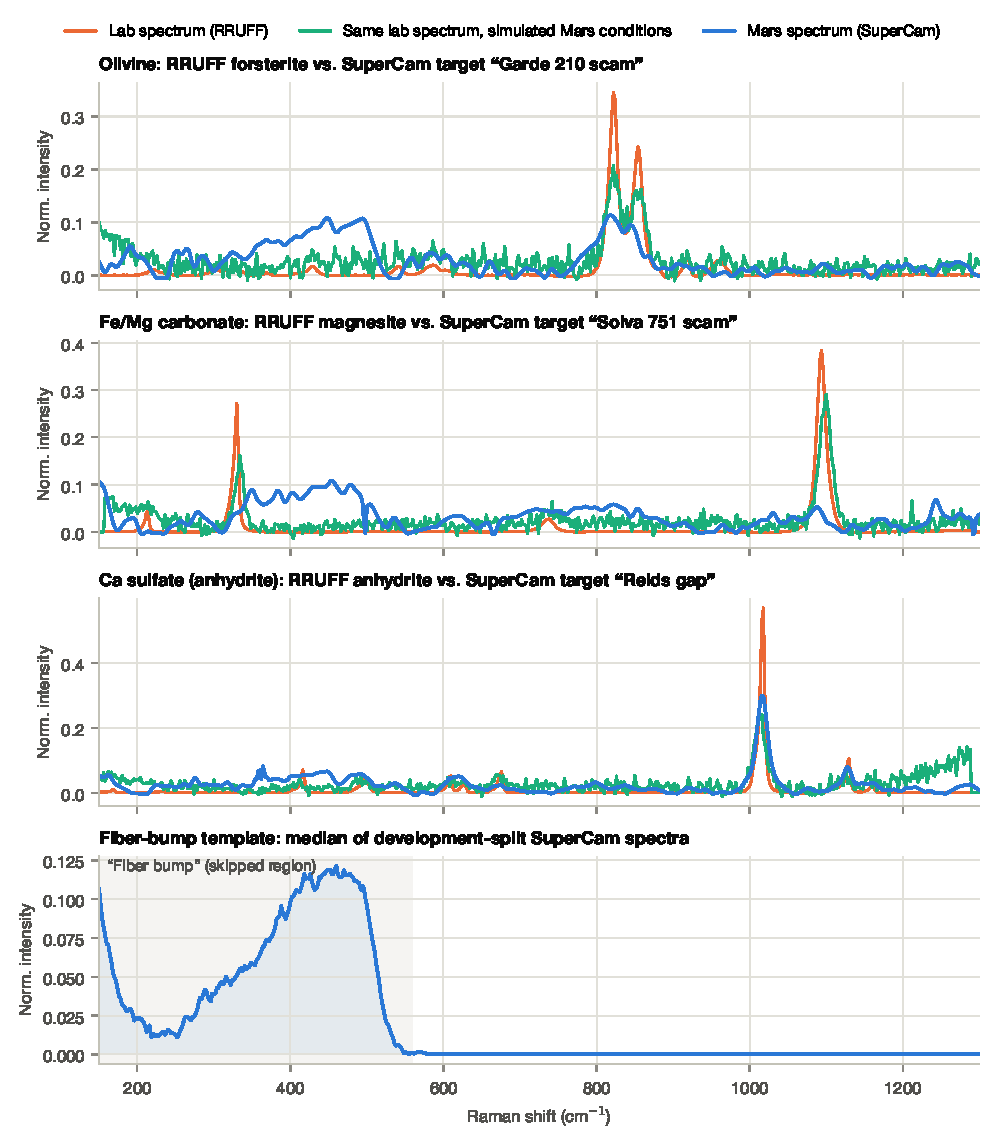
\includegraphics[width=0.82\linewidth]{figures/fig1_domain_gap.pdf}
\caption{\textbf{The lab-to-Mars gap.} Top three panels: a SuperCam spectrum (blue) for each of the three most common mineral groups, the matching RRUFF lab spectrum (orange), and the same lab spectrum after our simulated-Mars degradation (green). SuperCam peaks are broader and weaker relative to the background. Bottom: the median of the development-split SuperCam spectra, showing the broad ``fiber bump'' below about 560\,cm$^{-1}$ (shaded) that appears in most spectra whatever the mineral.}
\label{fig:gap}
\end{figure}

\subsection{In the lab, ``Shazam for minerals'' works}
On held-out lab samples, every method finds the right mineral group almost all the time: library search reaches \labGrpCleanCosineOpen{} group accuracy and \labSpCleanCosineOpen{} species accuracy across \nLabTestSpecies{} species. When the held-out lab spectra are degraded with our simulated-Mars effects, library search slips gradually, to \labGrpTwoCosineOpen{} group accuracy at twice the training strength. The CNN trained on simulated-Mars spectra is the most robust to these degradations (\labGrpTwoCnnMarsifiedOpen{} at strength 2; Figure~\ref{fig:simreal}a). If lab tests were the whole story, simulated-Mars training would look like a clear success.

\subsection{On Mars, the open library fails}
The picture changes completely on real SuperCam spectra (Table~\ref{tab:main}, Figure~\ref{fig:bars}). When predictions may be any RRUFF mineral, library search gets only \accCosineOpen{} of test spectra right (\balCosineOpen{} balanced accuracy), and no method exceeds \balCnnMarsifiedArtifactOpen{} balanced accuracy. The reason is easy to see in the matches. For \fracOtherOpen{} of Mars test spectra, the best library match is a mineral that is not in any group the team reports. For \fracAmorphOpen{}, it is a glass, opal, or other amorphous phase, led by synthetic rare-earth glasses and Libyan Desert glass. These materials have broad, featureless bands that resemble SuperCam's fiber bump, which on average carries \energyBumpMars{} of a Mars spectrum's normalized signal, compared with \energyBumpLab{} for lab spectra. The best cosine similarity is also lower on Mars (median \simMars{}) than between lab samples (median \simLab{}).

\begin{table}[!htbp]
\centering
\caption{\textbf{Main results.} Lab: mineral-group accuracy on held-out RRUFF samples (clean, open library; most held-out lab species lie outside the nine Mars groups, so the lab column is the same model scored without the Mars restriction). Mars: plain accuracy and balanced accuracy (mean recall over the six primary groups) on the \nMarsEval{} SuperCam test spectra, with 95\% cluster-bootstrap intervals over rocks. CNN numbers are three-seed ensembles. Bold: best balanced accuracy in each setting.}
\label{tab:main}
\small
\begin{tabular}{lcccc}
\toprule
 & Lab (clean) & \multicolumn{3}{c}{Mars test} \\
\cmidrule(lr){2-2}\cmidrule(lr){3-5}
Method & Group acc. & Acc. & Bal.\ acc. & 95\% CI (bal.) \\
\midrule
\multicolumn{5}{l}{\emph{Open library}}\\
Library search & 98\% & 5\% & 19\% & 2\%--24\%\\
\quad + skip fiber bump & 96\% & 6\% & 17\% & 1\%--21\%\\
\quad + resolution-matched & 98\% & 5\% & 21\% & 1\%--25\%\\
\quad + resolution-matched + skip & 95\% & 12\% & 28\% & 6\%--36\%\\
CNN, lab spectra & 98\% & 6\% & 26\% & 0\%--30\%\\
\quad + skip fiber bump & 98\% & 2\% & 7\% & 0\%--9\%\\
CNN, simulated-Mars training & 98\% & 7\% & 27\% & 2\%--31\%\\
\quad + skip fiber bump & 97\% & 5\% & 16\% & 2\%--20\%\\
\quad + fiber-bump template & 98\% & 13\% & \textbf{32\%} & 5\%--39\%\\
\addlinespace
\multicolumn{5}{l}{\emph{Mars-candidate library}}\\
Library search & 98\% & 45\% & 60\% & 33\%--66\%\\
\quad + skip fiber bump & 96\% & 68\% & \textbf{72\%} & 51\%--79\%\\
\quad + resolution-matched & 98\% & 38\% & 56\% & 29\%--63\%\\
\quad + resolution-matched + skip & 95\% & 62\% & 66\% & 46\%--73\%\\
CNN, lab spectra & 98\% & 44\% & 63\% & 44\%--68\%\\
\quad + skip fiber bump & 98\% & 38\% & 55\% & 30\%--62\%\\
CNN, simulated-Mars training & 98\% & 22\% & 48\% & 25\%--54\%\\
\quad + skip fiber bump & 97\% & 24\% & 40\% & 14\%--46\%\\
\quad + fiber-bump template & 98\% & 44\% & 58\% & 38\%--66\%\\
\addlinespace
Always ``olivine'' & -- & 50\% & 18\% & -- \\
\bottomrule
\end{tabular}

\end{table}

\begin{figure}[!htbp]
\centering
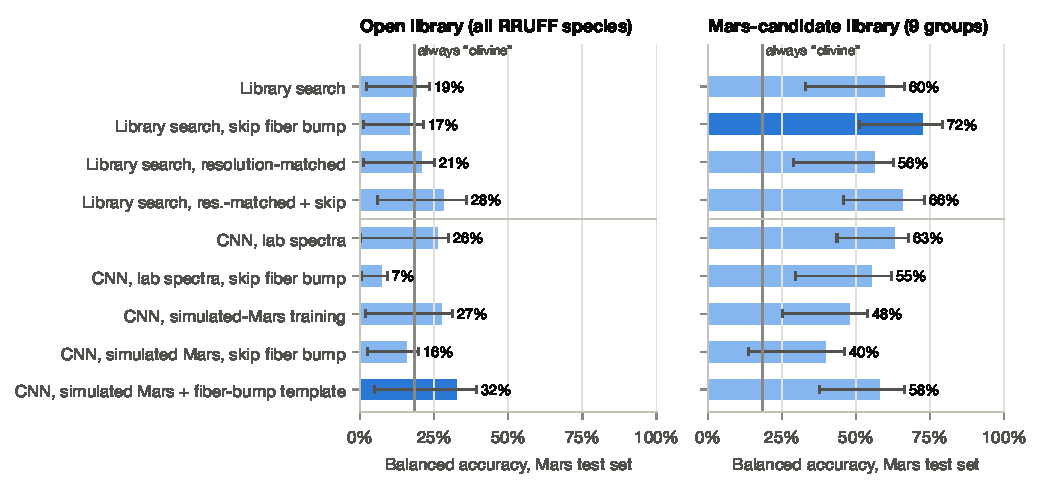
\includegraphics[width=\linewidth]{figures/fig2_mars_accuracy.pdf}
\caption{\textbf{Balanced accuracy on real SuperCam test spectra.} Left: predictions may be any RRUFF mineral. Right: predictions are restricted to the nine mineral groups reported in Jezero crater. Error bars are 95\% cluster-bootstrap intervals over rocks. The gray line is the trivial ``always olivine'' classifier. The darkest bar marks the best method in each panel.}
\label{fig:bars}
\end{figure}

\subsection{Prior knowledge and one simple fix recover most of the gap}
Restricting predictions to the Mars-candidate groups helps every method. Library search rises to \balCosineMars{} balanced accuracy (\accCosineMars{} accuracy). The single most effective change, however, is the simplest: skipping the fiber-bump region below 560\,cm$^{-1}$. With it, library search reaches \textbf{\balCosineWindowMars{}} balanced accuracy (95\% CI \balCICosineWindowMars{}) and \accCosineWindowMars{} accuracy, the highest score in this study. The gain over plain library search is \dWinVsCos{} percentage points (paired 95\% CI \dCIWinVsCos{}, $p=\pWinVsCos{}$). Its lead over the clean-lab CNN (\dWinVsCnn{} points, CI \dCIWinVsCnn{}, $p=\pWinVsCnn{}$) is not statistically significant with this test set, so we treat the two as roughly comparable, with library search ahead. The share of amorphous matches in the open setting falls from \fracAmorphOpen{} to \fracAmorphWindow{}. This choice is not an artifact of looking at the test set: on the development split, the skip variant is also the best library method (\devCosineWindow{} vs.\ \devCosine{} balanced accuracy) and beats the development-selected CNN (\devCnnClean{}). Per mineral, it identifies olivine in \recOlivineCosineWindowMars{} of cases and carbonate in \recCarbonateCosineWindowMars{} (Table~\ref{tab:recall}).

Matching the library to SuperCam's 12\,cm$^{-1}$ resolution, which one might expect to help, \emph{lowers} balanced accuracy both without the skip (\balCosineBroadenedMars{}) and with it (\balCosineBroadenedWindowMars{}). One possible explanation is that blurring makes many reference spectra look more alike, which costs more than the better peak-shape match gains.

\begin{table}[!htbp]
\centering
\caption{Recall per primary mineral group on the SuperCam test set (Mars-candidate setting).}
\label{tab:recall}
\small
\begin{tabular}{lcccccc}
\toprule
Method & Olivine & Carbonate & Sulfate & Pyroxene & Feldspar & Silica\\
 & ($n$=119) & ($n$=77) & ($n$=29) & ($n$=12) & ($n$=10) & ($n$=8)\\
\midrule
Library search & 36\% & 38\% & 79\% & 25\% & 80\% & 100\%\\
Library search, skip bump & 78\% & 58\% & 28\% & 100\% & 70\% & 100\%\\
Library search, res.-matched & 26\% & 34\% & 72\% & 25\% & 80\% & 100\%\\
Library search, res.-matched + skip & 68\% & 60\% & 24\% & 92\% & 50\% & 100\%\\
CNN, lab spectra & 29\% & 44\% & 72\% & 42\% & 90\% & 100\%\\
CNN, lab spectra, skip bump & 18\% & 48\% & 66\% & 50\% & 50\% & 100\%\\
CNN, simulated Mars & 5\% & 13\% & 79\% & 0\% & 90\% & 100\%\\
CNN, sim.\ Mars, skip bump & 21\% & 14\% & 34\% & 8\% & 60\% & 100\%\\
CNN, sim.\ Mars + template & 39\% & 38\% & 66\% & 17\% & 90\% & 100\%\\
\bottomrule
\end{tabular}

\end{table}

\subsection{Simulated-Mars training does not transfer to real Mars}
The CNN trained on clean lab spectra was selected on the development split. It reaches \balCnnCleanMars{} balanced accuracy on the test set (individual seeds: $\pm$\seedSdCnnCleanMars{} points standard deviation), close to plain library search but well below the skip variant. Our simulated-Mars training, which made the CNN the most robust model on degraded lab spectra, \emph{lowers} real-Mars balanced accuracy to \balCnnMarsifiedMars{}, a significant drop (\dCnnVsSim{} points for the clean-lab CNN, CI \dCICnnVsSim{}, $p=\pCnnVsSim{}$). Skipping the fiber bump does not rescue it (\balCnnMarsifiedWindowMars{}). Adding the fiber-bump template recovers part of the loss (\balCnnMarsifiedArtifactMars{}; \dTplVsSim{} points, CI \dCITplVsSim{}, not significant) and gives the best open-library score (\balCnnMarsifiedArtifactOpen{}), but it still does not beat the CNN trained on clean lab spectra. Figure~\ref{fig:simreal}b summarizes the mismatch: among our methods, accuracy under simulated Mars conditions does not predict accuracy on real Mars. If anything, the trend is negative.



\begin{figure}[!htbp]
\centering
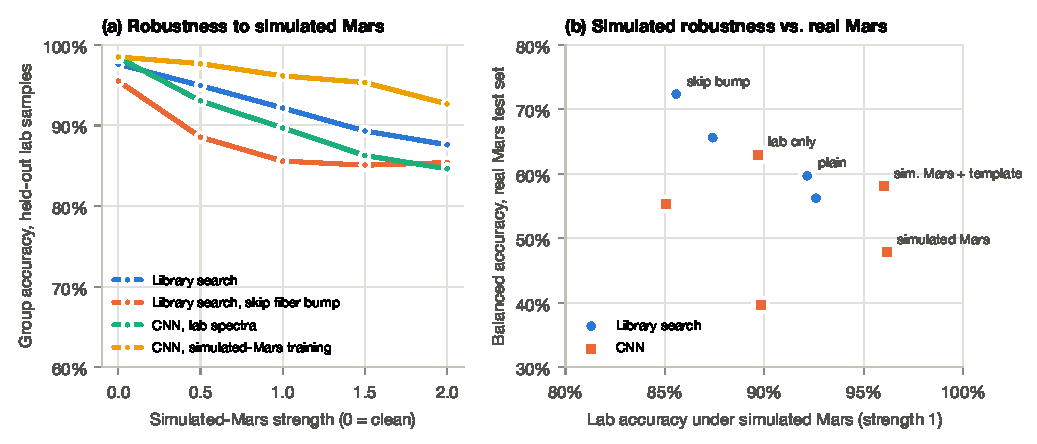
\includegraphics[width=\linewidth]{figures/fig3_sim_vs_real.pdf}
\caption{\textbf{Robustness to simulated Mars does not predict success on real Mars.} (a) Mineral-group accuracy on held-out lab spectra as the simulated-Mars degradation gets stronger (open-library setting). (b) For every method, lab accuracy under simulated Mars (strength 1) against balanced accuracy on the real SuperCam test set.}
\label{fig:simreal}
\end{figure}

\paragraph{Which simulated effect hurts?} To find out, we retrained the CNN with one simulated effect at a time (two seeds each; Figure~\ref{fig:single}). On the test set, \emph{every} single effect lowered balanced accuracy relative to no simulation (\seNoneTest{}): resolution blur \seResTest{}, calibration shift \seShiftTest{}, broad background \seBgTest{}, noise \seNoiseTest{}, and mineral mixing \seMixTest{}, the largest drop. All five together gave \seAllTest{}. Mixing was also the most harmful effect on the development split (\seMixDev{} vs.\ \seNoneDev{}). There, noise and background alone looked helpful (\seNoiseDev{} and \seBgDev{}), but the development split is small and the test set did not confirm this. One reading is that synthetic mixtures teach the network that a weak extra peak can be ignored, while on Mars weak peaks are often the signal itself.

\begin{figure}[!htbp]
\centering
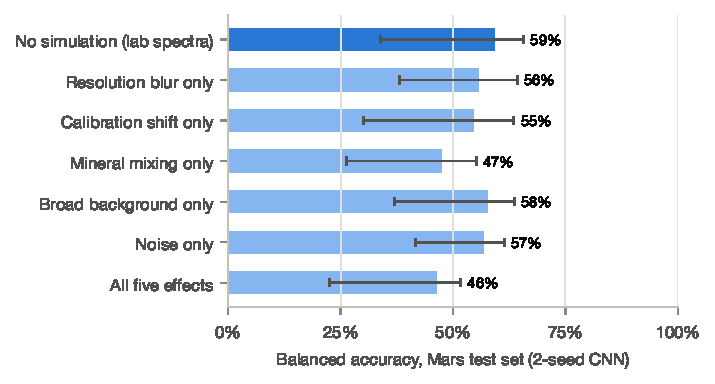
\includegraphics[width=0.7\linewidth]{figures/fig5_single_effects.pdf}
\caption{\textbf{One simulated effect at a time.} Balanced accuracy on the SuperCam test set (Mars-candidate setting) of CNNs trained with no simulation, with a single simulated-Mars effect, or with all five (two-seed ensembles; 95\% cluster-bootstrap intervals). The darkest bar marks training on clean lab spectra.}
\label{fig:single}
\end{figure}

\subsection{Where the errors are}
Figure~\ref{fig:confusion} shows the confusion patterns. Once the fiber bump is skipped, library search's remaining errors are mostly predictions of \emph{pyroxene}: for olivine, sulfate, and carbonate spectra alike, it is the most common wrong answer. Pyroxene's bands near 670 and 1010\,cm$^{-1}$ are broad on Mars and overlap anhydrite's main band at about 1017\,cm$^{-1}$. The clean-lab CNN instead tends to call olivine and carbonate spectra ``sulfate'' or ``feldspar''. Accuracy also follows the team's own confidence. For the skip variant, it is \confHighCW{} on high-confidence labels, \confMedCW{} on medium, and \confLowCW{} on low (\nConfHigh{}, \nConfMed{}, and \nConfLow{} spectra). The spectra that experts find hardest are hard for the algorithms too.

\begin{figure}[!htbp]
\centering
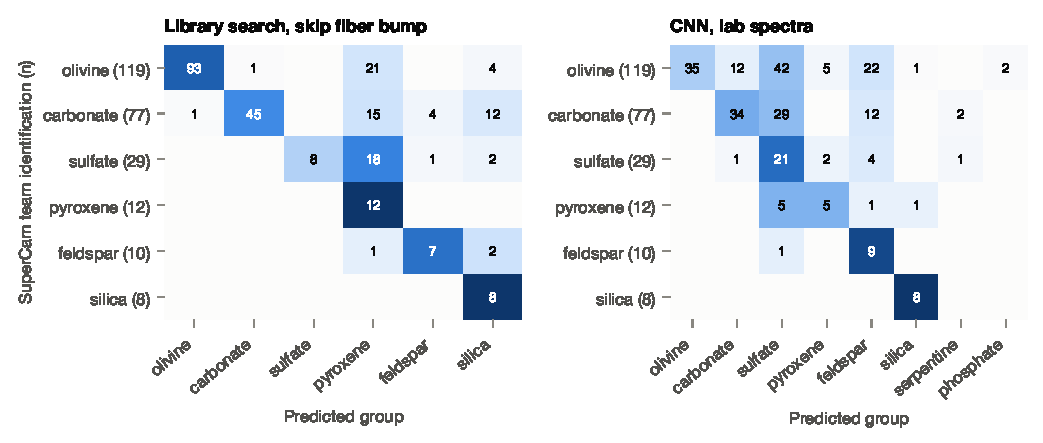
\includegraphics[width=\linewidth]{figures/fig4_confusion.pdf}
\caption{\textbf{Confusion matrices on the SuperCam test set} (Mars-candidate setting). Rows are the team's primary identification; a prediction that matches any group the team reported for that spectrum is counted on the diagonal. Cell color shows the fraction of the row.}
\label{fig:confusion}
\end{figure}

\FloatBarrier
\section{Discussion}
\label{sec:discussion}

\paragraph{Why the open library fails.} A big laboratory library is a strength in the lab and a liability on Mars. Among \nSpecies{} species there are always some, mostly glasses and other amorphous phases, whose broad bands fit SuperCam's broad fiber bump better than any crystalline mineral fits the weak, broadened Mars peaks. Nearest-neighbor matching has no way of knowing that the broadest feature in a Mars spectrum comes from the instrument. Two kinds of knowledge that mission scientists apply without thinking fix most of this: which minerals are plausible at the site, and which parts of the spectrum to trust. Encoding both explicitly took library search from \balCosineOpen{} to \balCosineWindowMars{} balanced accuracy.

\paragraph{The skip has a price.} Skipping the region below 560\,cm$^{-1}$ also throws away real mineral bands, such as quartz near 464\,cm$^{-1}$, feldspar near 480--510\,cm$^{-1}$, and the secondary anhydrite bands near 417 and 499\,cm$^{-1}$, all of which appear in the team's table. This shows up in the per-group recalls: skipping the region raises olivine recall from \recOlivineCosineMars{} to \recOlivineCosineWindowMars{} but lowers sulfate recall from \recSulfateCosineMars{} to \recSulfateCosineWindowMars{}, as anhydrite becomes easier to confuse with pyroxene in the 1000--1020\,cm$^{-1}$ region. A better treatment would model the fiber bump rather than delete the region. Our fiber-bump template is one attempt, and it helped the CNN (\balCnnMarsifiedArtifactMars{} vs.\ \balCnnMarsifiedMars{}) without solving the problem.

\paragraph{Simulated robustness is not real robustness.} The most important negative result of this study is that our simulated-Mars training worked as intended in the lab and hurt on Mars. That training is a reasonable recipe: blurring to the instrument's resolution, calibration shifts, mixing, smooth backgrounds, and noise. Two lessons follow. First, a degradation model is a hypothesis about the instrument, and a wrong hypothesis can teach a model to rely on the wrong cues. For example, a CNN trained on smooth synthetic backgrounds may learn to ignore exactly the kind of broad structure that the fiber bump adds, then misread it at test time. Second, evaluating Mars-oriented classifiers only on synthetically degraded lab spectra, as is often done, can give a misleading picture. Labeled flight spectra are the only way to check. This is the main reason we release the benchmark.

\paragraph{Simple and transparent does well.} The highest-scoring method in this study is also the simplest: cosine matching against a lab library, with a physically motivated restriction and mask. This agrees with earlier lab results in which full-spectrum similarity matching did as well as or better than trained classifiers \citep{carey2015machine}. It is also practical for mission use, because every decision can be traced to a specific reference spectrum. Deep models may still win with better training data, for example spectra from SuperCam-like laboratory systems \citep{manrique2024simulcam}, or with unsupervised domain adaptation on the thousands of unlabeled SuperCam spectra in the archive \citep{ganin2016domain}. Our results suggest that such methods should be judged on flight data, not on simulations.

\subsection{Limitations}
\label{sec:limits}
\paragraph{The labels are expert interpretations.} Our reference labels are the SuperCam team's identifications, not independent ground truth. Some are marked low confidence, and some lean on SuperCam's other techniques (LIBS and visible/infrared spectroscopy) as well as Raman. A model that ``disagrees'' with a low-confidence label is not necessarily wrong, which is why we also report results by confidence level (Section~\ref{sec:results}).

\paragraph{Only spectra with detectable minerals are included.} The team's table lists only spectra that contain identifiable mineral features \citep{jpl2026supercamsis}. Our test therefore asks ``\emph{which} mineral is this?'' and never ``is there a mineral signal here at all?''. A deployed system would also need to reject spectra with no usable signal, and our numbers say nothing about that.

\paragraph{Small, imbalanced, clustered data.} The test set has \nMarsEval{} spectra from only \nMarsTargets{} rocks. Olivine dominates it, and silica, feldspar, and pyroxene have only 8--12 spectra each. We report balanced accuracy and cluster-bootstrap confidence intervals over rocks, but the per-class numbers for the rarest groups are uncertain, and the intervals are wide.

\paragraph{Processing differs between the two domains.} The Mars spectra come already processed by the mission pipeline (despiking, denoising, response correction) \citep{jpl2026supercamsis}, while the RRUFF spectra come from several laboratory instruments and lasers. We apply the same baseline correction and normalization to both, but some differences remain, for example in relative peak heights between 532 and 785\,nm excitation.

\paragraph{Using unlabeled Mars spectra.} The fiber-bump template is estimated from unlabeled SuperCam spectra of the development split. This is legitimate unsupervised adaptation, since no labels or test spectra are used, but it does use real flight data. The ``simulated-Mars only'' CNN, which uses no Mars data at all, is the purer lab-to-Mars result.

\paragraph{What we did not try.} Lab instruments built to mimic SuperCam \citep{manrique2024simulcam} could provide more realistic training spectra. Domain-adversarial training \citep{ganin2016domain} could use the many unlabeled SuperCam spectra in the archive. The OH band near 3690\,cm$^{-1}$ would be needed to recognize serpentine and other hydrated minerals.


\section{Conclusion}
\label{sec:conclusion}
A ``Shazam for minerals'' built from Earth laboratory spectra does not work on Mars out of the box. Allowed to choose any mineral, it decides that most Perseverance SuperCam spectra are glass. Two pieces of expert knowledge fix most of the problem: restricting predictions to minerals known from Jezero crater, and ignoring the instrument's fiber bump. Together they bring a simple library search to \balCosineWindowMars{} balanced accuracy, and to \confHighCW{} on the spectra that the SuperCam team identified with high confidence. Training a neural network on simulated Mars conditions, by contrast, made it more robust in the lab and \emph{worse} on Mars. Lab-to-Mars transfer should therefore be measured on real flight data. The benchmark we release, built from public PDS data, makes that measurement possible for anyone.

\section*{Data and code availability}
All data are public. The RRUFF Raman spectra are available from \url{https://www.rruff.net} \citep{lafuente2015rruff}. The SuperCam calibrated spectra and the derived Raman identification table are in the Mars 2020 SuperCam bundle on the NASA PDS Geosciences Node \citep{wiens2021supercambundle}. The code that downloads the data, runs every experiment, and regenerates every figure, table, and number in this paper is available at \url{https://github.com/anartuvshinbayar/research-3}.

\section*{Use of AI tools}
% TODO (author): edit this statement so it accurately describes how you used AI, and check the
% target journal's policy before submitting.
The author used an AI assistant (Claude, Anthropic) to help write the analysis code, run the experiments, and draft the manuscript text. The author reviewed the code, results, and text, and takes full responsibility for the content. The AI tool is not an author.

\section*{Acknowledgments}
We thank the RRUFF project for its open mineral spectral database, and the Mars 2020 SuperCam team and the NASA Planetary Data System Geosciences Node for making SuperCam data and the team's Raman mineral identifications publicly available.


\bibliographystyle{unsrtnat}
\bibliography{refs}

\appendix
\section{Development history and additional results}
\label{app:history}

\paragraph{Two fixes made during development.} In the interest of transparency, we report two problems found while building the pipeline. Both were diagnosed on the development split and fixed before the final run reported in the main text.
\begin{enumerate}
\item \textbf{Mixed-anion minerals.} Our first chemistry rule labeled any RRUFF species containing CO$_3$ (or SO$_4$) as a carbonate (or sulfate), even if it also contained another oxyanion group. As a result, arsenate-bearing species such as beudantite and tyrolite were counted as sulfates or carbonates. Their strongest bands sit at 800--870\,cm$^{-1}$, on top of olivine's doublet, so they ``won'' many Mars olivine spectra. The corrected rule counts a species as a carbonate or sulfate only if it contains no other anion-forming element. The number of sulfate species fell from 191 to 141 and carbonate species from 138 to 111.
\item \textbf{How species probabilities become a group.} We first summed the CNN's species probabilities within each group. Under domain shift, a CNN spreads its probability across many species, so summing favors groups with many species (141 sulfates against 7 olivines). The final rule takes the group of the single most probable allowed species, the same rule library search uses. For the clean-lab CNN, summing gives \sumBalCnnCleanMars{} balanced accuracy, against \balCnnCleanMars{} with the final rule. For the CNN with simulated Mars and the fiber-bump template, the two rules give \sumBalCnnMarsifiedArtifactMars{} and \balCnnMarsifiedArtifactMars{}.
\end{enumerate}
An earlier version of the pipeline that contained both problems was also scored once on the test split. Its numbers are not reported because they reflect these errors. All configurations of the final pipeline that we evaluated are reported in Table~\ref{tab:main}.

\paragraph{Development-split scores.} On the \nDevEval{} development spectra (Mars-candidate setting), balanced accuracy was \devCosine{} for library search, \devCosineWindow{} for library search with the bump skipped, \devCnnClean{} for the clean-lab CNN (the CNN selected for the main text), \devCnnMarsified{} for the simulated-Mars CNN, and \devCnnMarsifiedArtifact{} for the simulated-Mars CNN with the template. The development split has few classes (no feldspar or silica), so these numbers are noisier than the test numbers. Still, both splits rank library search with the bump skipped first and the clean-lab CNN second, and both rank the simulated-Mars CNN last among these five.


\end{document}
